\chapter{Vergleich}
\label{chap:vergleich}

In diesem Kapitel werden numerische Ergebnisse
der beiden Verfahren f�r verschiedene Testprobleme
vorgestellt.
Wir beschr�nken unseren Test auf
Optimierungsprobleme mit linearen Restriktionen.
Wir werden somit Optimierungsprobleme
mit nichtlinearen Restriktionen
wegen des h�hen Aufwands
nicht ber�cksichtigen.

\section{Testprobleme}

Die Testprobleme k�nnen in drei Gruppen geteilt werden.
Die erste Gruppe besteht aus Problemen
\eqref{prob:opt_prob_mit_var_beschr}
mit nur oberen und unteren Schranken.
Zu der zweiten Gruppe geh�ren die Probleme
\eqref{prob:opt_prob_mit_lin_gl_nebenbed}
mit linearen Gleichungsnebenbedingungen.
Die Probleme \eqref{prob:opt_prob_mit_lin_ungl_nebenbed}
mit linearen Ungleichungsnebenbedingungen
kommen anschlie�end in die letzte Gruppe.

\begin{testproblem}
\begin{equation}
\min_{x\in\R^2}\ (x_1 - 4)^2 + (x_2 - 7)^2
\end{equation}
\begin{equation*}
\begin{split}
\nb -10 \leq x_i & \leq 10,\ i = 1,2 \\
\end{split}
\end{equation*}
\end{testproblem}

\begin{testproblem}
Rosenbrock-Funktion (vgl. Beispiel 1.4.1 in \cite[S.~14]{alt})
\begin{equation}
\min_{x\in\R^2}\ 100 (x_2-x_1^2)^2+(1-x_1)^2 
\end{equation}
\begin{equation*}
\begin{split}
\nb -10 \leq x_i & \leq 10,\ i = 1,2 \\
\end{split}
\end{equation*}
\end{testproblem}

\begin{testproblem}
Himmelblau-Funktion (vgl. Beispiel 1.4.2 in \cite[S.~14f]{alt})
\begin{equation}
\min_{x\in\R^2}\ (x_1^2+x_2-11)^2 + (x_1+x_2^2-7)^2 
\end{equation}
\begin{equation*}
\begin{split}
\nb -10 \leq x_i & \leq 10,\ i = 1,2 \\
\end{split}
\end{equation*}
\end{testproblem}

\begin{testproblem}
Bazaraa-Shetty-Funktion (vgl. Beispiel 1.4.3 in \cite[S.~15f]{alt})
\begin{equation}
\min_{x\in\R^2}\ (x_1-2)^4+(x_1-2 x_2)^2 
\end{equation}
\begin{equation*}
\begin{split}
\nb -10 \leq x_i & \leq 10,\ i = 1,2 \\
\end{split}
\end{equation*}
\end{testproblem}

\begin{testproblem}
(vgl. Beispiel 1.4.4 in \cite[S.~16]{alt})
\begin{equation}
\min_{x\in\R^2}\ (1.5-x_1 (1-x_2))^2+(2.25-x_1 (1-x_2^2))^2+(2.625-x_1 (1-x_2^3))^2 
\end{equation}
\begin{equation*}
\begin{split}
\nb -10 \leq x_i & \leq 10,\ i = 1,2 \\
\end{split}
\end{equation*}
\end{testproblem}

\begin{testproblem}
\begin{equation}
\min_{x\in\R^3}\ e^{\|x\|^2} 
\end{equation}
\begin{equation*}
\begin{split}
\nb -10 \leq x_i & \leq 10,\ i = 1,2,3 \\
\end{split}
\end{equation*}
\end{testproblem}

\begin{testproblem}
\begin{equation}
\begin{split}
  \min_{x\in\R^4}\ & 100(x_2-x_1^2)^2 + (1-x_1)^2 + 90(x_4-x_3^2)^2 + (1-x_3)^2\\
    & + 10.1((x_2-1)^2 + (x_4-1)^2) + 19.8(x_2-1)(x_4-1)
\end{split}
\end{equation}
\begin{equation*}
\begin{split}
\nb -10 \leq x_i & \leq 10,\ i = 1,\ldots,4 \\
\end{split}
\end{equation*}
\end{testproblem}

\begin{testproblem}
\begin{equation}
\min_{x\in\R^3}\ (x_1 - 4)^2 + (x_2 - 2)^2 + (x_3 - 7)^2
\end{equation}
\begin{equation*}
\begin{split}
\nb 5 \leq x_i & \leq 10,\ i = 1,2,3 \\
\end{split}
\end{equation*}
\end{testproblem}

\begin{testproblem}
\begin{equation}
\min_{x\in\R^2}\ 100 (x_2-x_1^2)^2+(1-x_1)^2 
\end{equation}
\begin{equation*}
\begin{split}
\nb -10 \leq x_1 & \leq 10 \\
1.5 \leq x_2 & \leq 10 \\
\end{split}
\end{equation*}
\end{testproblem}

\begin{testproblem}
\begin{equation}
\min_{x\in\R^2}\ (x_1^2+x_2-11)^2 + (x_1+x_2^2-7)^2 
\end{equation}
\begin{equation*}
\begin{split}
\nb -10 \leq x_1 & \leq 10 \\
5 \leq x_2 & \leq 10 \\
\end{split}
\end{equation*}
\end{testproblem}

\begin{testproblem}
\begin{equation}
\min_{x\in\R^2}\ (x_1-2)^4+(x_1-2 x_2)^2 
\end{equation}
\begin{equation*}
\begin{split}
\nb 4 \leq x_1 & \leq 10 \\
-10 \leq x_2 & \leq 10 \\
\end{split}
\end{equation*}
\end{testproblem}

\begin{testproblem}
(vgl. Beispiel 1.4.4 in \cite[S.~16]{alt})
\begin{equation}
\min_{x\in\R^2}\ (1.5-x_1 (1-x_2))^2+(2.25-x_1 (1-x_2^2))^2+(2.625-x_1 (1-x_2^3))^2 
\end{equation}
\begin{equation*}
\begin{split}
\nb 3 \leq x_1 & \leq 10 \\
-10 \leq x_2 & \leq 10 \\
\end{split}
\end{equation*}
\end{testproblem}

\begin{testproblem}
\begin{equation}
\min_{x\in\R^3}\ e^{\|x\|^2} 
\end{equation}
\begin{equation*}
\begin{split}
\nb 0.5 \leq x_1 & \leq 10 \\
1 \leq x_i & \leq 10,\ i = 2,3 \\
\end{split}
\end{equation*}
\end{testproblem}

\begin{testproblem}
\begin{equation}
\begin{split}
  \min_{x\in\R^4}\ & 100(x_2-x_1^2)^2 + (1-x_1)^2 + 90(x_4-x_3^2)^2 + (1-x_3)^2\\
    & + 10.1((x_2-1)^2 + (x_4-1)^2) + 19.8(x_2-1)(x_4-1)
\end{split}
\end{equation}
\begin{equation*}
\begin{split}
\nb 2 \leq x_1 & \leq 10 \\
-10 \leq x_i & \leq 10,\ i = 2,3,4 \\
\end{split}
\end{equation*}
\end{testproblem}

\begin{example}
\emph{(Lineare Regression, vgl. Beispiel 1.1.6 in \cite[S.~4f]{alt})}\\
Ein Beispiel unrestringiertes Optimierungsproblems ist
die Aufgabe der linearen Regression.
Gegeben seien m-Messwerte $(\xi_i,\eta_i), i = 1,\ldots,m$.
Gesucht ist eine Gerade
\begin{equation}
  \eta(\xi) := x_1 \xi + x_2,
\end{equation}
die \textss{optimal} zu den Messwerten passt.
D.\,h. wir sollen den Parameter $x = (x_1,x_2)^T \in \R^2$
so bestimmen, dass die Summe der Fehlerquadrate
in den Messpunkten minimiert wird.
Wir haben somit das Optimierungsproblem
\begin{equation}
  \min_{x \in \R^2}\ 
  f(x) := \sum_{i=1}^{m} (\eta(\xi_i) - \eta_i)^2
        = \sum_{i=1}^{m} (x_1 \xi_i + x_2 - \eta_i)^2.
\end{equation}
\end{example}

\begin{testproblem}
\label{test_prob:lin_regres}
Lineare Regression
\begin{equation}
\min_{x\in\R^2}\ \sum_{i=1}^{10} (x_1 \xi_i + x_2 - \eta_i)^2
\end{equation}
\begin{equation*}
\begin{split}
\nb -10 \leq x_i & \leq 10,\ i = 1,2 \\
\end{split}
\end{equation*}
Die Messwerte $(\xi_i,\eta_i), i = 1,\ldots,10,$
sind in der Tabelle~\ref{tbl:messwerte_lin_regres}
zu finden.
\end{testproblem}

\begin{table}[h]
\centering
\begin{tabular*}{0.8\linewidth}{@{\extracolsep{\fill}}c|cccccccccc}
  $\xi_i$ & 1 & 2 & 3 & 4 & 5 & 6 & 7 & 8 & 9 & 10 \\
  \midrule
  $\eta_i$ & $-0.5$ & $-2$ & $-3$ & $-3$ & $-2.5$
    & $-2$ & $-1$ & 1 & 3 & $5.5$ \\
\end{tabular*}
\caption{Messwerte f�r Testprobleme~\ref{test_prob:lin_regres}
und~\ref{test_prob:nichtlin_regres_quad}}
\label{tbl:messwerte_lin_regres}
\end{table}

\begin{example}
\emph{(Nichtlineare Regression, vgl. Abschnitt 2.3.2 in \cite[S.~30f]{alt})}\\
Neben linearen Regressionsaufgaben sind auch oft
nichtlineare Regressionsaufgaben zu l�sen.
Gesucht ist der funktionale Zusammenhang $\eta(\xi)$
zwischen den $\xi$- und den $\eta$-Werten,
beispielweise
\begin{equation}\label{eq:nichtlin_regres_quad_zusammenhang}
  \eta(\xi) := x_1 (\xi -x_2)^2 + x_3
\end{equation}
oder
\begin{equation}\label{eq:nichtlin_regres_exp_zusammenhang}
  \eta(\xi) := x_1 e^{\xi x_2}.
\end{equation}
Dabei ist $x = (x_1,\ldots,x_n)^T \in \R^n$ ein Parametervektor,
der \textss{optimal}
bestimmt werden soll.
\end{example}

\begin{testproblem}
\label{test_prob:nichtlin_regres_quad}
Nichtlineare Regression mit dem funktionalen
Zusammenhang~\eqref{eq:nichtlin_regres_quad_zusammenhang}
\begin{equation}
\min_{x\in\R^3}\ \sum_{i=1}^{10} (x_1 (\xi_i -x_2)^2 + x_3 - \eta_i)^2
\end{equation}
\begin{equation*}
\begin{split}
\nb -10 \leq x_i & \leq 20,\ i = 1,2,3 \\
\end{split}
\end{equation*}
Die Messwerte $(\xi_i,\eta_i), i = 1,\ldots,10,$
in der Tabelle~\ref{tbl:messwerte_lin_regres}
sind zu benutzen.
\end{testproblem}

\begin{figure}[h]
\centering
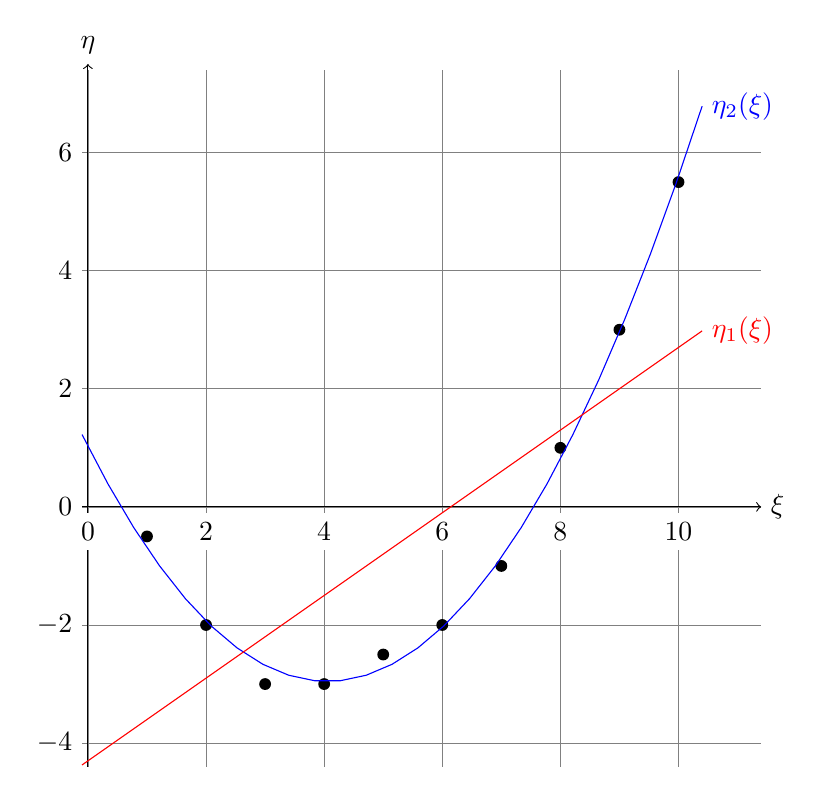
\begin{tikzpicture}[domain=-0.1:10.4,scale=0.75]
  \draw[very thin,color=gray,step=2] (-0.1,-4.4) grid (11.4,7.4);
  \draw[->] (-0.1,0) -- (11.4,0) node[right] {$\xi$};
  \draw[->] (0,-4.4) -- (0,7.5) node[above] {$\eta$};
  %\draw (-0.1,0.2) node [below left,fill=white] {0};
  \foreach \x in {0,2,4,...,10}
    \draw (\x,-0.1) node[below,fill=white] {$\x$};
  \foreach \y in {-4,-2,...,6}
    \draw (-0.1,\y) node[left] {$\y$};
  \foreach \x/\y in
    {1/-0.5, 2/-2, 3/-3, 4/-3, 5/-2.5, 6/-2, 7/-1, 8/1, 9/3, 10/5.5}
    \fill (\x,\y) circle(0.1);
  \draw[color=blue] plot (\x,{0.242*(\x-4.056)^2-2.955})
    node[right] {$\eta_2(\xi)$};
  \draw[color=red] plot (\x,{0.7*\x-4.3})
    node[right] {$\eta_1(\xi)$};
\end{tikzpicture}
\caption{L�sungen der Testprobleme~\ref{test_prob:lin_regres}
und~\ref{test_prob:nichtlin_regres_quad}}
\end{figure}

\begin{testproblem}
\label{test_prob:nichtlin_regres_exp}
Nichtlineare Regression mit dem funktionalen
Zusammenhang~\eqref{eq:nichtlin_regres_exp_zusammenhang}
\begin{equation}
\min_{x\in\R^2}\ \sum_{i=1}^{10} (x_1 e^{\xi x_2} - \eta_i)^2
\end{equation}
\begin{equation*}
\begin{split}
\nb -10 \leq x_i & \leq 10,\ i = 1,2 \\
\end{split}
\end{equation*}
Die Messwerte $(\xi_i,\eta_i), i = 1,\ldots,10,$
sind in der Tabelle~\ref{tbl:messwerte_nichtlin_regres}
gegeben.
\end{testproblem}

\begin{table}[h]
\centering
\begin{tabular*}{0.8\linewidth}{@{\extracolsep{\fill}}c|cccccccccc}
  $\xi_i$ & 1 & 2 & 3 & 4 & 5 & 6 & 7 & 8 & 9 & 10 \\
  \midrule
  $\eta_i$ & 1 & 1.1 & 1.2 & 1.35 & 1.55
    & 1.75 & 2.5 & 3 & 3.7 & 4.5 \\
\end{tabular*}
\caption{Messwerte f�r Testproblem~\ref{test_prob:nichtlin_regres_exp}}
\label{tbl:messwerte_nichtlin_regres}
\end{table}

\begin{testproblem}
(vgl. Beispiel 16.2 in \cite[S.~452]{nocedal}
\begin{equation}
\min_{x\in\R^3}\ \tfrac{1}{2} x^T Q x + q^T x + c
\end{equation}
\begin{equation*}
\begin{split}
\nb x_1 + x_3 & = 3 \\
x_2 + x_3 & = 0 \\
\end{split}
\end{equation*}
\end{testproblem}

\begin{testproblem}
\begin{equation}
\min_{x\in\R^5}\ \| x-x_d \|^2
\end{equation}
\begin{equation*}
\begin{split}
\nb x_1 + x_2 + x_3 + x_4 + x_5 & = 1 \\
\end{split}
\end{equation*}
\end{testproblem}

\begin{testproblem}
(vgl. Problem 28 in \cite[S.~51]{hock})
\begin{equation}
\min_{x\in\R^3}\ \tfrac{1}{2} x^T Q x + q^T x + c
\end{equation}
\begin{equation*}
\begin{split}
\nb x_1 + 2 x_2 + 3 x_3 & = 1 \\
\end{split}
\end{equation*}
\end{testproblem}

\begin{testproblem}
(vgl. Problem 48 in \cite[S.~71]{hock})
\begin{equation}
\min_{x\in\R^5}\ \tfrac{1}{2} x^T Q x + q^T x + c
\end{equation}
\begin{equation*}
\begin{split}
\nb x_1 + x_2 + x_3 + x_4 + x_5 & = 5 \\
x_3 - 2 x_4 - 2 x_5 & = -3 \\
\end{split}
\end{equation*}
\end{testproblem}

\begin{testproblem}
(vgl. Problem 51 in \cite[S.~74]{hock})
\begin{equation}
\min_{x\in\R^5}\ \tfrac{1}{2} x^T Q x + q^T x + c
\end{equation}
\begin{equation*}
\begin{split}
\nb x_1 + 3 x_2 & = 4 \\
x_3 + x_4 - 2 x_5 & = 0 \\
x_2 - x_5 & = 0 \\
\end{split}
\end{equation*}
\end{testproblem}

\begin{testproblem}
(vgl. Problem 52 in \cite[S.~75]{hock})
\begin{equation}
\min_{x\in\R^5}\ \tfrac{1}{2} x^T Q x + q^T x + c
\end{equation}
\begin{equation*}
\begin{split}
\nb x_1 + 3 x_2 & = 0 \\
x_3 + x_4 - 2 x_5 & = 0 \\
x_2 - x_5 & = 0 \\
\end{split}
\end{equation*}
\end{testproblem}

\begin{testproblem}
(vgl. Problem 53 in \cite[S.~76]{hock})
\begin{equation}
\min_{x\in\R^5}\ \tfrac{1}{2} x^T Q x + q^T x + c
\end{equation}
\begin{equation*}
\begin{split}
\nb x_1 + 3 x_2 & = 0 \\
x_3 + x_4 - 2 x_5 & = 0 \\
x_2 - x_5 & = 0 \\
-10 \leq x_i & \leq 10,\ i = 1,\ldots,5 \\
\end{split}
\end{equation*}
\end{testproblem}

\begin{testproblem}
(vgl. Problem 49 in \cite[S.~72]{hock})
\begin{equation}
\min_{x\in\R^5}\ (x_1-x_2)^2 + (x_3-1)^2 + (x_4-1)^2 + (x_5-1)^6 
\end{equation}
\begin{equation*}
\begin{split}
\nb x_1 + x_2 + x_3 + 4 x_4 & = 7 \\
x_3 + 5 x_5 & = 6 \\
\end{split}
\end{equation*}
\end{testproblem}

\begin{testproblem}
(vgl. Problem 50 in \cite[S.~73]{hock})
\begin{equation}
\min_{x\in\R^5}\ (x_1-x_2)^2 + (x_2-x_3)^2 + (x_3-x_4)^4 + (x_4-x_5)^2 
\end{equation}
\begin{equation*}
\begin{split}
\nb x_1 + 2 x_2 + 3 x_3 & = 6 \\
x_2 + 2 x_3 + 3 x_4 & = 6 \\
x_3 + 2 x_4 + 3 x_5 & = 6 \\
\end{split}
\end{equation*}
\end{testproblem}

\begin{testproblem}
\begin{equation}
\min_{x\in\R^2}\ \tfrac{1}{2} x^T Q x + q^T x + c
\end{equation}
\begin{equation*}
\begin{split}
\nb 2 x_1 + x_2 & \leq 2 \\
x_1 - x_2 & \leq 1 \\
-x_1 - x_2 & \leq 1 \\
-2 x_1 + x_2 & \leq 2 \\
\end{split}
\end{equation*}
\end{testproblem}

\begin{testproblem}
(vgl. Beispiel 16.4 in \cite[S.~475]{nocedal})
\begin{equation}
\min_{x\in\R^2}\ \| x-x_d \|^2
\end{equation}
\begin{equation*}
\begin{split}
\nb -x_1 + 2 x_2 & \leq 2 \\
x_1 + 2 x_2 & \leq 6 \\
x_1 - 2 x_2 & \leq 2 \\
0 & \leq x_i,\ i = 1,2 \\
\end{split}
\end{equation*}
\end{testproblem}

\begin{testproblem}
(vgl. Beispiel 13.2 in \cite[S.~415f]{antoniou})
\begin{equation}
\min_{x\in\R^4}\ \tfrac{1}{2} x^T Q x + q^T x + c
\end{equation}
\begin{equation*}
\begin{split}
\nb -x_1 & \leq 0 \\
-x_2 & \leq 0 \\
x_1 + 2 x_2 & \leq 2 \\
-x_4 & \leq -2 \\
-x_3 - x_4 & \leq -3 \\
x_3 + 2 x_4 & \leq 6 \\
\end{split}
\end{equation*}
\end{testproblem}

\begin{testproblem}
(vgl. Problem 21 in \cite[S.~44]{hock})
\begin{equation}
\min_{x\in\R^2}\ \tfrac{1}{2} x^T Q x + q^T x + c
\end{equation}
\begin{equation*}
\begin{split}
\nb -10 x_1 + x_2 & \leq -10 \\
2 \leq x_1 & \leq 50 \\
-50 \leq x_2 & \leq 50 \\
\end{split}
\end{equation*}
\end{testproblem}

\begin{testproblem}
(vgl. Problem 35 in \cite[S.~58]{hock})
\begin{equation}
\min_{x\in\R^3}\ \tfrac{1}{2} x^T Q x + q^T x + c
\end{equation}
\begin{equation*}
\begin{split}
\nb x_1 + x_2 + 2 x_3 & \leq 3 \\
0 & \leq x_i,\ i = 1,2,3 \\
\end{split}
\end{equation*}
\end{testproblem}

\begin{testproblem}
(vgl. Problem 76 in \cite[S.~96]{hock})
\begin{equation}
\min_{x\in\R^4}\ \tfrac{1}{2} x^T Q x + q^T x + c
\end{equation}
\begin{equation*}
\begin{split}
\nb x_1 + 2 x_2 + x_3 + x_4 & \leq 5 \\
3 x_1 + x_2 + 2 x_3 - x_4 & \leq 4 \\
-x_2 - 4 x_3 & \leq -1.5 \\
0 & \leq x_i,\ i = 1,\ldots,4 \\
\end{split}
\end{equation*}
\end{testproblem}




\begin{testproblem}
L�se folgendes, einfaches, 2-dimensionales Problem.
\begin{align}
  \min_{x \in \R^2}\ (x_1 - 1)^2 + (x_2 &- 2.5)^2 \\
  \nb -x_1 + 2x_2 & \leq 2 \\
       x_1 + 2x_2 & \leq 6 \\
       x_1 - 2x_2 & \leq 6 \\
                0 & \leq x_1, x_2
\end{align}
\end{testproblem}

\begin{figure}[ht]
\centering
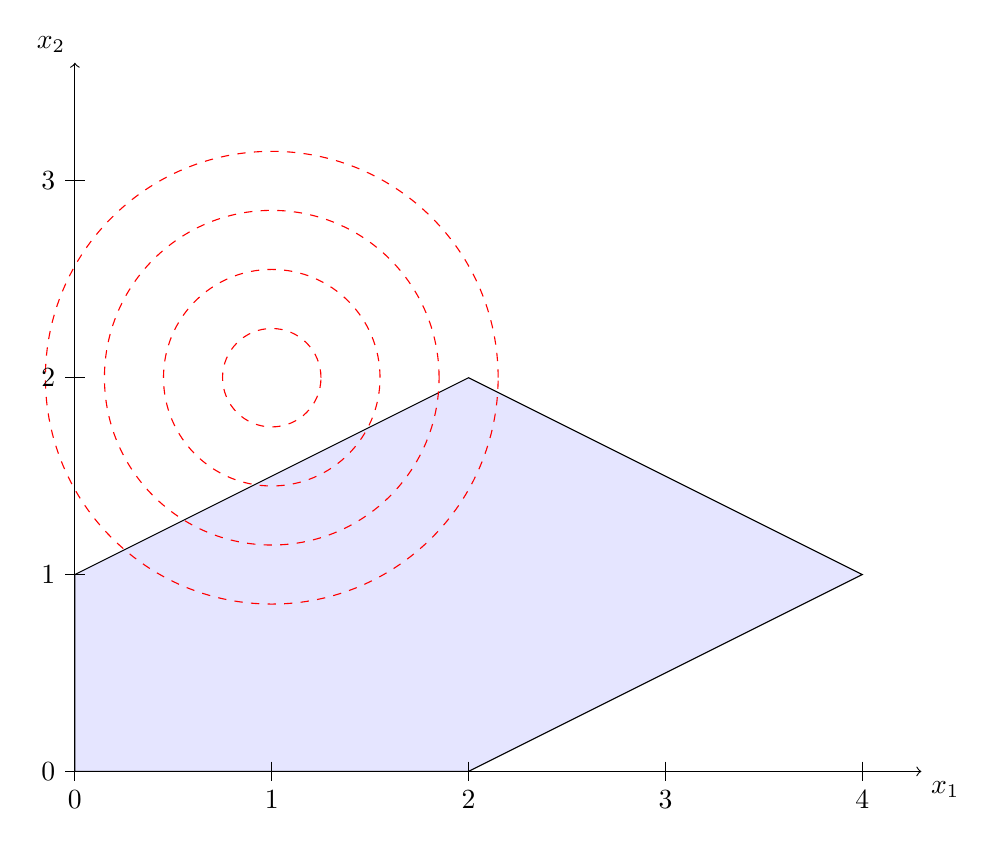
\begin{tikzpicture}[scale=2.5]
  
  % Die zul�ssige Menge
  \draw[fill=blue!10] (0,0) -- (0,1) -- (2,2) -- (4,1) -- (2,0) -- cycle;
  \draw (1.7,1) node {$\F$};
  
  % Die Niveaulinien
  \foreach \r in {0.25, 0.55, 0.85, 1.15}
    \draw[dashed,color=red] (1,2) circle (\r);
  
  % Koordinatenachsen
  \draw[->] (0,0) -- (4.3,0) node [below right] {$x_1$};
  \foreach \x in {0,...,4}
    \draw (\x,0.05) -- (\x,-0.05) node [below] {\x};
  \draw[->] (0,0) -- (0,3.6) node [above left] {$x_2$};
  \foreach \y in {0,...,3}
    \draw (0.05,\y) -- (-0.05,\y) node [left] {\y};
  
\end{tikzpicture}
\caption{Restringiertes Problem}
\end{figure}




\section{Numerische Ergebnisse}

\begin{table}[h]
\centering
\begin{tabular*}{0.5\linewidth}{@{\extracolsep{\fill}}crr}
  \toprule
  Testproblem &   SSN   &   SQP   \\
  \cmidrule{2-3}
              & \multicolumn{2}{c}{T (ms)} \\
  \midrule
  1 & 17.5 & 17.5 \\ % test_problem_v_norm
  2 & 22.5 & 37.34 \\ % test_problem_v_rosenbrock
  3 & 23.91 & 40.0 \\ % test_problem_v_himmelblau
  4 & 62.03 & 134.69 \\ % test_problem_v_bazaraa_shetty
  5 & 67.66 & 83.75 \\ % test_problem_v_beale
  6 & 205.62 & 355.31 \\ % test_problem_v_exp
  7 & 592.03 & 659.22 \\ % test_problem_v_colville
  8 & 15.78 & 19.84 \\ % test_problem_v_norm_1
  9 & 22.97 & 51.25 \\ % test_problem_v_rosenbrock_1
  10 & 23.59 & 80.62 \\ % test_problem_v_himmelblau_1
  11 & 19.38 & 23.28 \\ % test_problem_v_bazaraa_shetty_1
  12 & 81.88 & 80.31 \\ % test_problem_v_beale_1
  13 & 206.41 & 374.53 \\ % test_problem_v_exp_1
  14 & 267.5 & 328.28 \\ % test_problem_v_colville_1
  15 & 62.5 & 72.5 \\ % test_problem_v_lin_regression
  16 & 680.94 & 741.88 \\ % test_problem_v_quad_regression
  17 & 412.03 & 490.78 \\ % test_problem_v_nichtlin_regression
  \bottomrule
\end{tabular*}
\caption{Laufzeiten der Programme f�r Testprobleme 1 bis 17}
\end{table}

\begin{table}[h]
\centering
\begin{tabular*}{0.5\linewidth}{@{\extracolsep{\fill}}crr}
  \toprule
  Testproblem &   SSN   &   SQP   \\
  \cmidrule{2-3}
              & \multicolumn{2}{c}{T (ms)} \\
  \midrule
  18 & 15.62 & 15.78 \\ % test_problem_A_example_16_2_nocedal_wright
  19 & 16.09 & 15.62 \\ % test_problem_A_simple_example
  20 & 16.41 & 15.94 \\ % test_problem_A_huang_aggerwal_hs28
  21 & 16.09 & 16.88 \\ % test_problem_A_huang_aggerwal_miele_hs48
  22 & 15.62 & 15.62 \\ % test_problem_A_huang_aggerwal_hs51
  23 & 15.94 & 16.25 \\ % test_problem_A_miele_hs52
  24 & 17.03 & 18.28 \\ % test_problem_Av_betts_miele_hs53
  25 & 67.81 & 73.91 \\ % test_problem_A_huang_aggerwal_hs49
  26 & 232.5 & 265.31 \\ % test_problem_A_huang_aggerwal_hs50
  \bottomrule
\end{tabular*}
\caption{Laufzeiten der Programme f�r Testprobleme 18 bis 26}
\end{table}

\begin{table}[h]
\centering
\begin{tabular*}{0.5\linewidth}{@{\extracolsep{\fill}}crr}
  \toprule
  Testproblem &   SSN   &   SQP   \\
  \cmidrule{2-3}
              & \multicolumn{2}{c}{T (ms)} \\
  \midrule
  27 & 16.09 & 18.75 \\ % test_problem_G_example_with_diamond_area
  28 & 15.62 & 19.84 \\ % test_problem_Gv_example_16_4_nocedal_wright
  29 & 15.94 & 31.09 \\ % test_problem_G_example_13_2_antoniou_lu
  30 & 16.41 & 17.66 \\ % test_problem_Gv_betts_hs21
  31 & 15.78 & 16.25 \\ % test_problem_Gv_beale_hs35
  32 & 16.41 & 42.34 \\ % test_problem_Gv_murtagh_sargent_hs76
  33 & 20.94 & 27.19 \\ % test_problem_AG_opt_ctrl
  \bottomrule
\end{tabular*}
\caption{Laufzeiten der Programme f�r Testprobleme 27 bis 33}
\end{table}

